% =========================================================
% The Triangle Inequality: One Picture, All Consequences
% =========================================================

\subsubsection{The Triangle Inequality: One Picture, All Consequences}
\label{sec:triangle-inequality-geometry}

\begin{remark*}[Triangle inequality as a proof tool]
The triangle inequality is not only a geometric axiom of metrics;
it is also one of the principal algebraic tools used in analysis.
Later we will see how it allows complicated expressions to be
bounded by decomposing them into simpler distances.
Typical applications include limit laws for sums, products,
and quotients of sequences.
\end{remark*}

Recall the definitions
\[
B_r(x) \;:=\; \{y\in X : d(x,y)<r\},
\qquad
\overline{B}_r(x) \;:=\; \{y\in X : d(x,y)\le r\}.
\]

Every metric space $(X,d)$ postulates the triangle inequality as one of
its defining axioms:
\[
\forall\,x,y,z \in X,\qquad d(x,z) \;\le\; d(x,y) + d(y,z).
\]
This single statement has more consequences than it first appears.
All three ``sides'' of a triangle give inequalities by the same axiom,
and rearranging any one of them yields the \emph{reverse triangle
inequality}, which controls how rapidly distances can change.
Both facts flow from a single geometric picture.

% ---- Toolkit ----------------------------------------------------------------------------------------------------
\begin{tcolorbox}[colback=gray!6, colframe=gray!40, arc=2pt,
  left=6pt, right=6pt, top=4pt, bottom=4pt,
  title={\small\textbf{Triangle Inequality --- Quick Reference}},
  fonttitle=\small\bfseries]
\small
\begin{tabular}{l l l}
\toprule
\textbf{Name} & \textbf{Statement} & \textbf{Detail} \\
\midrule
Triangle inequality (M4)
  & $d(x,z) \le d(x,y)+d(y,z)$
  & \hyperref[prop:triangle-three-forms]{$\downarrow$} \\
Three symmetric forms
  & all sides $\le$ sum of other two
  & \hyperref[prop:triangle-three-forms]{$\downarrow$} \\
Reverse triangle inequality
  & $|d(x,z)-d(y,z)| \le d(x,y)$
  & \hyperref[prop:reverse-triangle]{$\downarrow$} \\
Interior ball identity
  & $y\!\in\!B_r(x)\Rightarrow B_{r-d(x,y)}(y)\!\subseteq\! B_r(x)$
  & \hyperref[rem:interior-ball-identity]{$\downarrow$} \\
Open ball as union of closed balls
  & $B_r(x)=\bigcup_{0<s<r}\overline{B}_s(x)$
  & \hyperref[prop:open-as-union-closed]{$\downarrow$} \\
Closed ball as intersection of open balls
  & $\overline{B}_r(x)=\bigcap_{\varepsilon>0}B_{r+\varepsilon}(x)$
  & \hyperref[prop:closed-as-int-open]{$\downarrow$} \\
\bottomrule
\end{tabular}
\end{tcolorbox}

% =========================================================
%  THE CORE PICTURE
% =========================================================

\subsubsection*{The Single Geometric Picture}

Fix three points $x, y, z \in X$.
Label the three pairwise distances as the sides of a triangle:

\bigskip
% figure-triangle-inequality-core.tex
% Triangle inequality: three forms, one geometric picture
% Requires:
%   \usepackage{tikz}
%   \usetikzlibrary{arrows.meta,positioning,calc}

\begin{center}
\begin{tikzpicture}[
  dot/.style={circle,fill,inner sep=2.0pt},
  lbl/.style={font=\small},
  slbl/.style={font=\scriptsize},
  >=stealth
]

% ---- Vertices ------------------------------------------------------------------------------------------------
% Place as a clear scalene triangle (not isoceles, to avoid suggesting
% special cases)
\coordinate (X) at (0,    0);
\coordinate (Y) at (4.2,  0);
\coordinate (Z) at (1.3,  2.6);

% ---- Filled triangle ----------------------------------------------------------------------------------
\fill[blue!6] (X) -- (Y) -- (Z) -- cycle;

% ---- Sides ------------------------------------------------------------------------------------------------------
% Bottom: x-y   [blue, the "base"]
\draw[blue!60!black, line width=1.2pt] (X) -- (Y);
% Left:   x-z   [orange]
\draw[orange!70!black, line width=1.2pt] (X) -- (Z);
% Right:  y-z   [red]
\draw[red!60!black, line width=1.2pt] (Y) -- (Z);

% ---- Points ----------------------------------------------------------------------------------------------------
\node[dot, fill=blue!65!black]   at (X) {};
\node[dot, fill=orange!70!black] at (Z) {};
\node[dot, fill=red!60!black]    at (Y) {};

% ---- Point labels ------------------------------------------------------------------------------------------
\node[lbl, anchor=north east] at ($(X)+(-0.05,-0.12)$) {$x$};
\node[lbl, anchor=north west] at ($(Y)+( 0.05,-0.12)$) {$y$};
\node[lbl, anchor=south]      at ($(Z)+( 0.00, 0.12)$) {$z$};

% ---- Side labels --------------------------------------------------------------------------------------------
% Bottom side x-y: label below
\node[slbl, text=blue!65!black, anchor=north]
  at ($(X)!0.5!(Y) + (0,-0.14)$)
  {$d(x,y)$};

% Left side x-z: label to the left
\node[slbl, text=orange!70!black, anchor=east]
  at ($(X)!0.5!(Z) + (-0.16,0)$)
  {$d(x,z)$};

% Right side y-z: label to the right
\node[slbl, text=red!60!black, anchor=west]
  at ($(Y)!0.5!(Z) + (0.16,0)$)
  {$d(y,z)$};

% ---- Three inequality callouts ------------------------------------------------------------------
% Placed outside each vertex, pointing to "which side is bounded"
\node[
  draw=orange!50, fill=orange!6, rounded corners=3pt,
  font=\scriptsize, inner sep=4pt, anchor=south east
] at (-0.4, 3.1) {
  $\textcolor{orange!70!black}{d(x,z)}
   \le d(x,y) + d(y,z)$
};
\draw[orange!50, ->, thin] (-0.38,3.05) -- ($(X)!0.42!(Z)+(-0.05,0.1)$);

\node[
  draw=blue!40, fill=blue!5, rounded corners=3pt,
  font=\scriptsize, inner sep=4pt, anchor=north
] at (2.1, -0.72) {
  $\textcolor{blue!65!black}{d(x,y)}
   \le d(x,z) + d(z,y)$
};

\node[
  draw=red!40, fill=red!5, rounded corners=3pt,
  font=\scriptsize, inner sep=4pt, anchor=south west
] at (4.65, 3.1) {
  $\textcolor{red!60!black}{d(y,z)}
   \le d(y,x) + d(x,z)$
};
\draw[red!40, ->, thin] (4.63,3.05) -- ($(Y)!0.45!(Z)+(0.05,0.1)$);

\end{tikzpicture}
\end{center}
\bigskip

\noindent
The triangle inequality (Axiom M4) is stated for one specific ordering
of the three points.
But the metric axioms also guarantee \emph{symmetry} ($d(x,y)=d(y,x)$),
so the same axiom applied with the points in each of the three possible
roles yields three inequalities, one bounding each side.

% =========================================================
%  PROPOSITION: THREE FORMS
% =========================================================

\begin{proposition}[\texorpdfstring{%
  \hyperref[prf:triangle-three-forms]{Three Forms of the Triangle Inequality}%
}{Three Forms of the Triangle Inequality}]
\label{prop:triangle-three-forms}
Let $(X,d)$ be a metric space and let $x,y,z\in X$.
Each side of the triangle is bounded by the sum of the other two:
\begin{align}
d(x,z) &\;\le\; d(x,y) + d(y,z), \label{tri:xz} \\
d(x,y) &\;\le\; d(x,z) + d(z,y), \label{tri:xy} \\
d(y,z) &\;\le\; d(y,x) + d(x,z). \label{tri:yz}
\end{align}
\end{proposition}

\begin{remark*}[Derivation from M4 and symmetry]
Axiom M4 is exactly \eqref{tri:xz}.
Applying M4 with the role of $y$ played by $z$ and vice versa gives
$d(x,y) \le d(x,z)+d(z,y)$, which is \eqref{tri:xy}.
Applying M4 with the points relabelled as $y,x,z$ (i.e.\ the ``first''
point is $y$) gives $d(y,z)\le d(y,x)+d(x,z)$, which is \eqref{tri:yz}.
Symmetry ($d(y,x)=d(x,y)$, $d(z,y)=d(y,z)$) makes each form a simple
rewriting of the others.
\end{remark*}

\begin{remark*}[One picture produces all three]
Each inequality says the same thing: \emph{any side of the triangle is
at most the sum of the other two sides.}
In Euclidean geometry this is obvious --- a straight line is the shortest
path.
In an abstract metric space there are no lines, but the axiom encodes
exactly this constraint.
\end{remark*}

% =========================================================
%  THE REVERSE TRIANGLE INEQUALITY
% =========================================================

\subsubsection*{Where the Reverse Triangle Inequality Comes From}

Rearranging \eqref{tri:xz} gives one half of the reverse inequality.
Then swapping the roles of $x$ and $y$ gives the other half.
Together they force the absolute value bound.

\bigskip
% figure-reverse-triangle-inequality.tex
% Reverse triangle inequality: derivation steps as callouts
% Requires:
%   \usepackage{tikz}
%   \usetikzlibrary{arrows.meta,positioning,calc}

\begin{center}
\begin{tikzpicture}[
  dot/.style={circle,fill,inner sep=2.0pt},
  lbl/.style={font=\small},
  slbl/.style={font=\scriptsize},
  >=stealth
]

% ---- Vertices (same scalene triangle) --------------------------------------------------
\coordinate (X) at (0,   0);
\coordinate (Y) at (4.2, 0);
\coordinate (Z) at (1.3, 2.6);

\fill[blue!6] (X) -- (Y) -- (Z) -- cycle;
\draw[blue!55!black,   line width=1.1pt] (X) -- (Y);
\draw[orange!65!black, line width=1.1pt] (X) -- (Z);
\draw[red!55!black,    line width=1.1pt] (Y) -- (Z);

\node[dot, fill=blue!65!black]   at (X) {};
\node[dot, fill=orange!65!black] at (Z) {};
\node[dot, fill=red!60!black]    at (Y) {};

\node[lbl, anchor=north east] at ($(X)+(-0.05,-0.12)$) {$x$};
\node[lbl, anchor=north west] at ($(Y)+( 0.05,-0.12)$) {$y$};
\node[lbl, anchor=south]      at ($(Z)+( 0.00, 0.12)$) {$z$};

\node[slbl, text=blue!60!black, anchor=north]
  at ($(X)!0.5!(Y)+(0,-0.14)$) {$d(x,y)$};
\node[slbl, text=orange!65!black, anchor=east]
  at ($(X)!0.5!(Z)+(-0.16,0)$) {$d(x,z)$};
\node[slbl, text=red!55!black, anchor=west]
  at ($(Y)!0.5!(Z)+(0.16,0)$) {$d(y,z)$};

% ---- Derivation steps as callouts ----------------------------------------------------------
% Step 1: rearrange d(x,z) \le d(x,y)+d(y,z)
\node[
  draw=gray!40, fill=gray!5, rounded corners=3pt,
  font=\scriptsize, text width=5.4cm, align=left, inner sep=5pt,
  anchor=north west
] at (5.0, 3.0) {
  \textbf{Step 1.} Rearrange \eqref{tri:xz}:\\[3pt]
  $d(x,z) \le d(x,y) + d(y,z)$\\[2pt]
  $\Rightarrow\; d(x,z)-d(y,z) \le d(x,y)$
};

% Step 2: swap x \leftrightarrow y
\node[
  draw=gray!40, fill=gray!5, rounded corners=3pt,
  font=\scriptsize, text width=5.4cm, align=left, inner sep=5pt,
  anchor=north west
] at (5.0, 1.55) {
  \textbf{Step 2.} Swap $x\leftrightarrow y$ in \eqref{tri:xy}:\\[3pt]
  $d(y,z) \le d(y,x) + d(x,z)$\\[2pt]
  $\Rightarrow\; d(y,z)-d(x,z) \le d(x,y)$
};

% Step 3: combine
\node[
  draw=violet!40, fill=violet!5, rounded corners=3pt,
  font=\scriptsize, text width=5.4cm, align=left, inner sep=5pt,
  anchor=north west
] at (5.0, 0.2) {
  \textbf{Combine:}\\[3pt]
  $\pm\bigl(d(x,z)-d(y,z)\bigr) \le d(x,y)$\\[2pt]
  $\Rightarrow\; |d(x,z)-d(y,z)| \le d(x,y)$
};

% Arrow from triangle to Step 1
\draw[gray!50, ->, thin] (4.0, 1.5) -- (5.0, 2.55);
% Arrow from triangle to Step 2
\draw[gray!50, ->, thin] (4.0, 1.5) -- (5.0, 1.28);

\end{tikzpicture}
\end{center}
\bigskip

\begin{proposition}[\texorpdfstring{%
  \hyperref[prf:reverse-triangle]{Reverse Triangle Inequality}%
}{Reverse Triangle Inequality}]
\label{prop:reverse-triangle}
Let $(X,d)$ be a metric space and let $x,y,z\in X$.
Then
\[
\bigl|\,d(x,z) - d(y,z)\,\bigr| \;\le\; d(x,y).
\]
\end{proposition}

\begin{remark*}[Proof shape]
From \eqref{tri:xz}: $d(x,z)\le d(x,y)+d(y,z)$, so
$d(x,z)-d(y,z)\le d(x,y)$.
From \eqref{tri:xy} with the roles of $x$ and $y$ swapped:
$d(y,z)\le d(y,x)+d(x,z)$, so $d(y,z)-d(x,z)\le d(x,y)$.
These two inequalities say $\pm(d(x,z)-d(y,z))\le d(x,y)$, which is
exactly $|d(x,z)-d(y,z)|\le d(x,y)$.
\end{remark*}

\begin{remark*}[Fully quantified form]
\[
\forall\,x,y,z\in X:\quad
\bigl|\,d(x,z)-d(y,z)\,\bigr| \;\le\; d(x,y).
\]
\end{remark*}

% ---- Intuition callout ----------------------------------------------------------------------------------
\begin{tcolorbox}[colback=propbox, colframe=propborder, arc=2pt,
  left=8pt, right=8pt, top=6pt, bottom=6pt]
\noindent\textbf{Intuition.}\quad
Fix $z$ and ask how the distance $d(\cdot\,,z)$ to $z$ changes as you
move from $x$ to $y$.
The reverse triangle inequality says:
\[
\text{the change in distance to }z \;\;\le\;\; d(x,y).
\]
Distances cannot change faster than you move.
No matter how far $z$ is from both $x$ and $y$, and no matter what
curved or abstract path the metric defines, the difference
$|d(x,z)-d(y,z)|$ is always bounded by the direct distance $d(x,y)$
between the two vantage points.
This is the geometric content encoded in all three triangle forms at once.
\end{tcolorbox}

\begin{remark*}[Consequence for continuity]
The reverse triangle inequality immediately shows that the distance
function $d : X \times X \to \mathbb{R}$ is continuous with respect to
any product metric on $X \times X$.
If $(x_n, y_n) \to (x, y)$ in the product, then
$|d(x_n, y_n) - d(x,y)| \le d(x_n,x) + d(y_n,y) \to 0$,
where the first step applies the reverse inequality twice.
\end{remark*}

\begin{remark*}[Consequence: equivalent metrics have related balls]
If two metrics $d$ and $d'$ on $X$ satisfy $d \le C \cdot d'$ for some
constant $C > 0$, then for all $x\in X$ and $r>0$,
\[
B^{d'}_{r/C}(x) \;\subseteq\; B^d_r(x).
\]
Balls in the stronger metric $d$ contain corresponding balls in $d'$
with rescaled radius.
This is the key tool for proving metric equivalence from ball-containment
conditions.
\end{remark*}

% =========================================================
%  INTERIOR BALL IDENTITY
% =========================================================

\subsubsection*{The Interior Ball Identity}

The triangle inequality gives a precise quantitative statement
about how much room an interior point has inside an open ball.
This single fact underlies the standard proofs that open balls
are open and that closed balls are closed.

\begin{remark*}[Interior ball identity]
\label{rem:interior-ball-identity}
Let $(X,d)$ be a metric space, $x\in X$, and $r>0$.
If $y\in B_r(x)$, define the \emph{radial gap} of $y$ in $B_r(x)$ by
\[
\delta \;:=\; r - d(x,y) \;>\; 0.
\]
Then $B_\delta(y) \subseteq B_r(x)$, i.e.\
\[
B_{r-d(x,y)}(y) \;\subseteq\; B_r(x).
\]
The radial gap $\delta$ measures how much room remains before the
inequality $d(x,\cdot) < r$ is violated; it is a lower bound on the
distance from $y$ to the complement:
\[
d\bigl(y,\, X\setminus B_r(x)\bigr) \;\ge\; \delta \;=\; r - d(x,y).
\]
(Equality need not hold in general metric spaces.)
\end{remark*}

\bigskip
% figure-radial-gap-interior-ball.tex
% Radial gap: inner ball B_{r-d(x,y)}(y) inside B_r(x)
% Requires:
%   \usepackage{tikz}
%   \usetikzlibrary{arrows.meta,positioning,calc}

\begin{center}
\begin{tikzpicture}[
  dot/.style={circle,fill,inner sep=1.8pt},
  >=stealth,
  lbl/.style={font=\small},
  slbl/.style={font=\scriptsize},
]

% ---- Coordinates ---------------------------------------------------------------
\coordinate (x)  at (0, 0);
\coordinate (y)  at (1.5, 0.5);

\def\R{3.2}     % radius of B_r(x)
% d(x,y) = sqrt(1.5^2 + 0.5^2) = sqrt(2.5) approx 1.58
% inner radius = R - d(x,y) approx 1.62   (fits comfortably inside)
\pgfmathsetmacro{\dxy}{sqrt(1.5*1.5+0.5*0.5)}   % approx 1.58
\pgfmathsetmacro{\inner}{\R - \dxy}               % approx 1.62

% ---- Outer ball B_r(x) ---------------------------------------------------------
\fill[blue!7]  (x) circle (\R);
\draw[blue!55!black, line width=1.3pt, dashed] (x) circle (\R);

% ---- Inner ball B_{r-d(x,y)}(y) -----------------------------------------------
\fill[orange!18] (y) circle (\inner);
\draw[orange!65!black, line width=1.1pt] (y) circle (\inner);

% ---- Points -------------------------------------------------------------------
\node[dot, fill=blue!65!black]   at (x) {};
\node[dot, fill=orange!70!black] at (y) {};

% ---- Point labels -------------------------------------------------------------
\node[lbl, anchor=north] at ($(x)+(0,-0.14)$) {$x$};
\node[lbl, anchor=south] at ($(y)+(0,0.12)$)  {$y$};

% ---- d(x,y) segment -----------------------------------------------------------
\draw[blue!60!black, line width=0.9pt] (x) -- (y);
\node[slbl, text=blue!60!black, anchor=north]
  at ($(x)!0.5!(y)+(0,-0.12)$) {$d(x,y)$};

% ---- Radius r (rightward) -----------------------------------------------------
\draw[blue!50!black, line width=0.8pt, <->]
  ($(x)+(0,-0.7)$) -- ++({\R},0)
  node[midway, slbl, below, yshift=-3pt, text=blue!55!black] {$r$};

% ---- Inner radius r-d(x,y) (upward from y) ------------------------------------
\draw[orange!60!black, line width=0.8pt, <->]
  (y) -- ++(0,{\inner})
  node[midway, slbl, right, xshift=3pt, text=orange!70!black]
  {$\delta = r - d(x,y)$};

% ---- Boundary point along x->y ray --------------------------------------------
\pgfmathsetmacro{\ux}{1.5/\dxy}
\pgfmathsetmacro{\uy}{0.5/\dxy}
\pgfmathsetmacro{\bx}{\ux*\R}
\pgfmathsetmacro{\by}{\uy*\R}
\node[dot, fill=blue!40!black, inner sep=1.0pt] at (\bx,\by) {};

% ---- Ball labels ---------------------------------------------------------------
\node[lbl, text=blue!60!black, font=\small\itshape]
  at (-2.3, 2.1) {$B_r(x)$};
\node[lbl, text=orange!65!black, font=\small\itshape]
  at ($(y)+(1.1,-1.3)$) {$B_{r-d(x,y)}(y)$};

% ---- Annotation ---------------------------------------------------------------
\node[slbl, text=gray!55!black, font=\scriptsize\itshape, anchor=north]
  at (0,-2.35)
  {radial gap $\delta = r - d(x,y) > 0$: room for $B_\delta(y)$ inside $B_r(x)$};

\end{tikzpicture}
\end{center}
\bigskip

\begin{remark*}[Symmetric radial gap identities]
The radial gap has a mirror form for exterior points.
Two formulas appear in all standard ball proofs:
\[
\begin{array}{ll}
\textbf{Inside }B_r(x): & \delta \;=\; r - d(x,y) \;>\; 0,
  \quad B_\delta(y)\subseteq B_r(x). \\[6pt]
\textbf{Outside }\overline{B}_r(x): & \delta \;=\; d(x,y) - r \;>\; 0,
  \quad B_\delta(y)\subseteq X\setminus\overline{B}_r(x).
\end{array}
\]
In both cases $\delta$ measures the gap in the relevant inequality ---
$r - d(x,y)$ in the first case, $d(x,y) - r$ in the second --- and
provides a safe radius around $y$.
The second identity follows from the reverse triangle inequality:
if $d(y,z) < \delta = d(x,y) - r$ then
\[
d(x,z) \;\ge\; d(x,y) - d(y,z) \;>\; r,
\]
so $z\notin\overline{B}_r(x)$.
\end{remark*}

% =========================================================
%  DUAL BALL PROPOSITIONS
% =========================================================

\subsubsection*{The Dual Ball Identities}

The interior ball identity has two global consequences that reveal how
open and closed balls approximate each other from opposite directions.
Together they express the same principle: \emph{interior points are those
with a positive radial gap in the inequality $d(x,\cdot)<r$.}

\begin{proposition}[\texorpdfstring{%
  \hyperref[prf:open-as-union-closed]{Open Ball as a Union of Closed Balls}%
}{Open Ball as a Union of Closed Balls}]
\label{prop:open-as-union-closed}
Let $(X,d)$ be a metric space, $x\in X$, and $r>0$.
Then
\[
B_r(x) \;=\; \bigcup_{0 < s < r} \overline{B}_s(x).
\]
\end{proposition}

\begin{proof}
($\supseteq$)\;
If $y\in\overline{B}_s(x)$ for some $s<r$, then $d(x,y)\le s<r$, so
$y\in B_r(x)$.

($\subseteq$)\;
If $y\in B_r(x)$, then $d(x,y)<r$.
Choose $s = \tfrac{d(x,y)+r}{2}$.
Then $d(x,y) < s < r$, so $y\in\overline{B}_s(x)$ and that closed ball
appears in the union.
\end{proof}

\begin{remark*}[How to read this]
Every point strictly inside the open ball belongs to some closed ball
whose radius is strictly between $d(x,y)$ and $r$.
The union is \emph{increasing}: as $s$ grows toward $r$ from below, the
closed balls $\overline{B}_s(x)$ grow and exhaust $B_r(x)$.
(In some metric spaces $B_r(x) = \overline{B}_s(x)$ may already hold
for some $s < r$, e.g.\ in discrete metrics.)
\end{remark*}

\begin{proposition}[\texorpdfstring{%
  \hyperref[prf:closed-as-int-open]{Closed Ball as an Intersection of Open Balls}%
}{Closed Ball as an Intersection of Open Balls}]
\label{prop:closed-as-int-open}
Let $(X,d)$ be a metric space, $x\in X$, and $r>0$.
Then
\[
\overline{B}_r(x) \;=\; \bigcap_{\varepsilon > 0} B_{r+\varepsilon}(x).
\]
\end{proposition}

\begin{proof}
($\subseteq$)\;
If $y\in\overline{B}_r(x)$, then $d(x,y)\le r < r+\varepsilon$ for every
$\varepsilon>0$, so $y\in B_{r+\varepsilon}(x)$ for every $\varepsilon>0$.
Hence $y$ belongs to the intersection.

($\supseteq$)\;
Suppose $y$ lies in the intersection, so $d(x,y)<r+\varepsilon$ for every
$\varepsilon>0$.
If $d(x,y)>r$, choose $\varepsilon = \tfrac{d(x,y)-r}{2}$.
Then $r+\varepsilon = \tfrac{r+d(x,y)}{2} < d(x,y)$, contradicting
$y\in B_{r+\varepsilon}(x)$.
Therefore $d(x,y)\le r$ and $y\in\overline{B}_r(x)$.
\end{proof}

\begin{remark*}[How to read this]
A point belongs to the closed ball if and only if it cannot escape any
open ball of radius slightly larger than $r$.
The intersection is \emph{decreasing}: as $\varepsilon\to 0^+$, the
open balls $B_{r+\varepsilon}(x)$ shrink toward $\overline{B}_r(x)$,
recovering it exactly in the limit.
\end{remark*}

% ---- Dual figure ---------------------------------------------------------------

\bigskip
% figure-dual-balls-union-intersection.tex
% Dual ball identities: open ball as union of closed, closed as intersection of open
% Requires:
%   \usepackage{tikz}
%   \usetikzlibrary{arrows.meta,positioning,calc}

\begin{center}
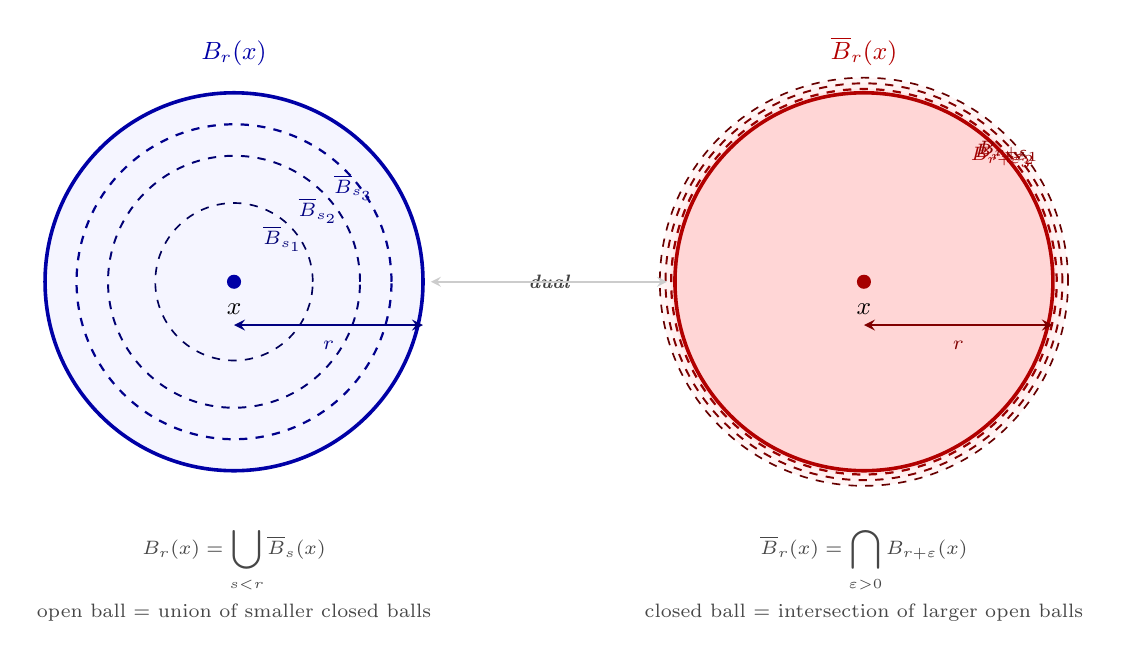
\begin{tikzpicture}[
  dot/.style={circle,fill,inner sep=1.8pt},
  >=stealth,
  lbl/.style={font=\small},
  slbl/.style={font=\scriptsize},
]

% ===== LEFT PANEL: B_r(x) = union of closed balls ================================
\begin{scope}[xshift=-4.0cm]

\def\R{2.4}

% Shaded closed balls at s=0.8, 1.4, 1.9 (building up the open ball)
\fill[blue!14] (0,0) circle (1.9);
\fill[blue!9]  (0,0) circle (2.15);
% The open ball itself
\fill[blue!4]  (0,0) circle (\R);

% Draw closed balls at three radii (dashed)
\draw[blue!35!black, line width=0.6pt, dashed] (0,0) circle (1.0);
\draw[blue!45!black, line width=0.7pt, dashed] (0,0) circle (1.6);
\draw[blue!55!black, line width=0.8pt, dashed] (0,0) circle (2.0);

% Outer open ball boundary (solid)
\draw[blue!65!black, line width=1.3pt] (0,0) circle (\R);

% Center
\node[dot, fill=blue!65!black] at (0,0) {};
\node[lbl, anchor=north] at (0,-0.16) {$x$};

% Radius r arrow
\draw[blue!50!black, <->, line width=0.75pt]
  (0,-0.55) -- ({\R},{ -0.55})
  node[midway, below, slbl, yshift=-2pt] {$r$};

% Closing ball labels
\node[slbl, text=blue!45!black] at (0.62, 0.55) {$\overline{B}_{s_1}$};
\node[slbl, text=blue!50!black] at (1.07, 0.90) {$\overline{B}_{s_2}$};
\node[slbl, text=blue!55!black] at (1.52, 1.20) {$\overline{B}_{s_3}$};

% Title
\node[lbl, text=blue!65!black, font=\small\itshape, anchor=south]
  at (0, {\R+0.22}) {$B_r(x)$};

\end{scope}

% ===== RIGHT PANEL: B̄_r(x) = intersection of open balls ========================
\begin{scope}[xshift=4.0cm]

\def\R{2.4}

% Draw open balls at three radii (dashed, getting smaller toward r)
\fill[red!4]  (0,0) circle ({1.08*\R});
\fill[red!6]  (0,0) circle ({1.05*\R});
\fill[red!10] (0,0) circle ({1.02*\R});

% Closed ball interior (solid fill)
\fill[red!16] (0,0) circle (\R);

% Open ball boundaries
\draw[red!40!black, line width=0.6pt, dashed] (0,0) circle ({1.08*\R});
\draw[red!50!black, line width=0.7pt, dashed] (0,0) circle ({1.05*\R});
\draw[red!60!black, line width=0.8pt, dashed] (0,0) circle ({1.02*\R});

% Closed ball boundary (solid)
\draw[red!70!black, line width=1.3pt] (0,0) circle (\R);

% Center
\node[dot, fill=red!65!black] at (0,0) {};
\node[lbl, anchor=north] at (0,-0.16) {$x$};

% Radius r arrow
\draw[red!50!black, <->, line width=0.75pt]
  (0,-0.55) -- ({\R},{-0.55})
  node[midway, below, slbl, yshift=-2pt] {$r$};

% Open ball labels at offsets
\node[slbl, text=red!55!black] at ({1.065*\R*0.72}, {1.065*\R*0.65}) {$B_{r+\varepsilon_1}$};
\node[slbl, text=red!60!black] at ({1.038*\R*0.72}, {1.038*\R*0.65}) {$B_{r+\varepsilon_2}$};
\node[slbl, text=red!65!black] at ({1.012*\R*0.72}, {1.012*\R*0.65}) {$B_{r+\varepsilon_3}$};

% Closed ball label
\node[lbl, text=red!70!black, font=\small\itshape, anchor=south]
  at (0,{\R+0.22}) {$\overline{B}_r(x)$};

\end{scope}

% ===== Central label ===========================================================
\node[slbl, text=gray!50!black, font=\scriptsize\itshape]
  at (0, 0) {\textbf{dual}};
\draw[gray!40, <->, line width=0.6pt] (-1.5, 0) -- (1.5, 0);

% ===== Captions below both panels (in outer scope, fixed y) ====================
\node[slbl, text=gray!55!black, anchor=north, align=center]
  at (-4.0, -3.0) {$B_r(x)=\displaystyle\bigcup_{s<r}\overline{B}_s(x)$\\[3pt]
                   open ball = union of smaller closed balls};
\node[slbl, text=gray!55!black, anchor=north, align=center]
  at ( 4.0, -3.0) {$\overline{B}_r(x)=\displaystyle\bigcap_{\varepsilon>0}B_{r+\varepsilon}(x)$\\[3pt]
                   closed ball = intersection of larger open balls};

\end{tikzpicture}
\end{center}
\bigskip

% ---- Unifying intuition -------------------------------------------------------
\begin{tcolorbox}[colback=propbox, colframe=propborder, arc=2pt,
  left=8pt, right=8pt, top=6pt, bottom=6pt]
\noindent\textbf{Unifying principle.}\quad
All results in this section reduce to one measurement: the
\emph{radial gap} of a point $y$ relative to a ball $B_r(x)$,
\[
\delta \;:=\; r - d(x,y).
\]
When $\delta > 0$ (i.e.\ $y\in B_r(x)$), the gap provides room for a
ball $B_\delta(y)$ entirely inside $B_r(x)$.
When $\delta < 0$ (i.e.\ $y\notin\overline{B}_r(x)$), the quantity
$-\delta = d(x,y)-r > 0$ provides room for a ball entirely outside
$\overline{B}_r(x)$.
In both cases the radial gap is a lower bound on the distance to the
complement:
\[
d\bigl(y,\,X\setminus B_r(x)\bigr) \;\ge\; r - d(x,y)
\quad\text{when } y\in B_r(x).
\]
\end{tcolorbox}

\begin{remark*}[Preview: distance to a set]
The radial gap $r - d(x,y)$ is a special case of the general concept
of \emph{distance from a point to a set}.
For $A\subseteq X$ define
\[
d(y,A) \;:=\; \inf_{a\in A}\, d(y,a).
\]
A point $y$ lies in the interior of a set $A$ if and only if
\[
d(y,\, X\setminus A) \;>\; 0.
\]
The radial gap satisfies $d(y, X\setminus B_r(x)) \ge r - d(x,y)$, so
positive radial gap implies positive distance to the complement ---
exactly the interior condition.
This formulation will reappear in the study of open and closed sets,
continuity, and compactness.
\end{remark*}

\begin{remark*}[Preview: balls form a basis]
Open balls form a basis for the metric topology: a set $U\subseteq X$ is open
iff for every $x\in U$ there exists $r>0$ such that
\[
B_r(x)\subseteq U.
\]
\end{remark*}